\begin{tikzpicture}[node distance=3cm]

\node (start) [startstop] {Start};
\node (in1) [io, below of=start] {read temprature};
\node (pro4) [process, below of=in1] {Display on LCD};
\node (dec1) [decision, below of=pro4, yshift=0.5cm] {is T>Threshold?};
\node (pro2b) [process, right of=dec1, xshift=2cm] {turn on the fan};
\node (pro3) [process, below of=dec1] {turn off the fan};
\node (stop) [startstop, below of=pro3] {Stop};


\draw [arrow] (start) -- (in1);
\draw [arrow] (in1) -- (pro4);
\draw [arrow] (pro4) -- (dec1);
\draw [arrow] (dec1) -- node[anchor=east] {yes} (pro2b);
\draw [arrow] (dec1) -- node[anchor=south] {no} (pro3);
\draw [arrow] (dec1) -- (pro2b);
\draw [arrow] (dec1) -- (pro3);
\draw [arrow] (pro3) -- (stop);

\end{tikzpicture}

\section{Circuit Diagram}

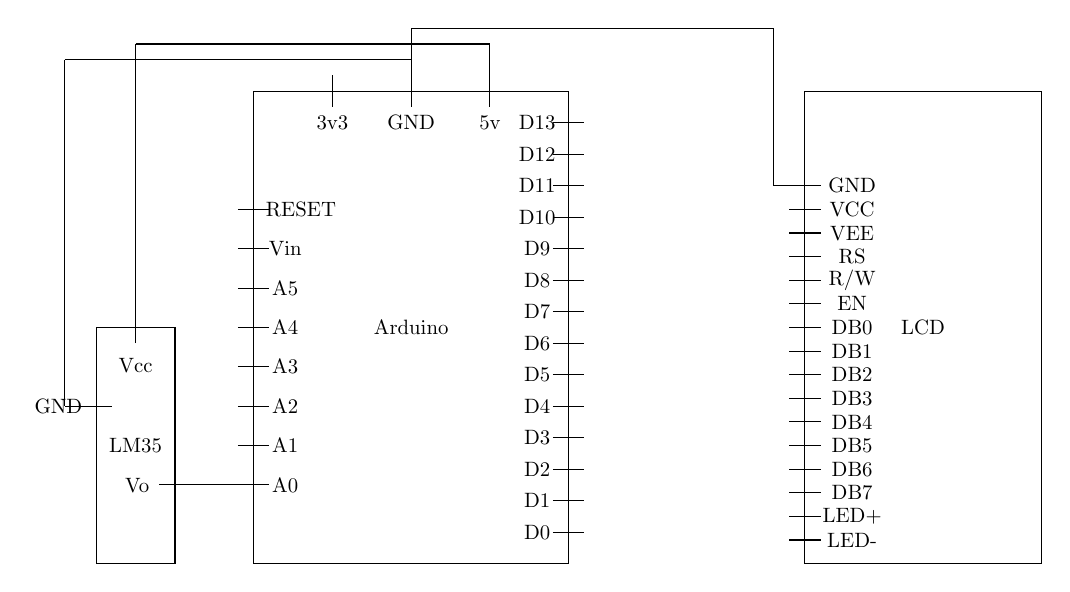
\begin{tikzpicture}
\draw (0,0) rectangle (4,6)node[pos=0.5, scale=0.75]{Arduino};

\draw (3.8,0.4) -- (4.2,0.4)node[pos=-0.5, scale=0.75]{D0};
\draw (3.8,0.8) -- (4.2,0.8)node[pos=-0.5, scale=0.75]{D1};
\draw (3.8,1.2) -- (4.2,1.2)node[pos=-0.5, scale=0.75]{D2};
\draw (3.8,1.6) -- (4.2,1.6)node[pos=-0.5, scale=0.75]{D3};
\draw (3.8,2.0) -- (4.2,2.0)node[pos=-0.5, scale=0.75]{D4};
\draw (3.8,2.4) -- (4.2,2.4)node[pos=-0.5, scale=0.75]{D5};
\draw (3.8,2.8) -- (4.2,2.8)node[pos=-0.5, scale=0.75]{D6};
\draw (3.8,3.2) -- (4.2,3.2)node[pos=-0.5, scale=0.75]{D7};
\draw (3.8,3.6) -- (4.2,3.6)node[pos=-0.5, scale=0.75]{D8};
\draw (3.8,4.0) -- (4.2,4.0)node[pos=-0.5, scale=0.75]{D9};
\draw (3.8,4.4) -- (4.2,4.4)node[pos=-0.5, scale=0.75]{D10};
\draw (3.8,4.8) -- (4.2,4.8)node[pos=-0.5, scale=0.75]{D11};
\draw (3.8,5.2) -- (4.2,5.2)node[pos=-0.5, scale=0.75]{D12};
\draw (3.8,5.6) -- (4.2,5.6)node[pos=-0.5, scale=0.75]{D13};
\draw (1,5.8) -- (1,6.2)node[pos=-0.5, scale=0.75]{3v3};
\draw (2,5.8) -- (2,6.2)node[pos=-0.5, scale=0.75]{GND};
\draw (3,5.8) -- (3,6.2)node[pos=-0.5, scale=0.75]{5v};
\draw (-0.2,1) -- (0.2,1)node[pos=1.5, scale=0.75]{A0};
\draw (-0.2,1.5) -- (0.2,1.5)node[pos=1.5, scale=0.75]{A1};
\draw (-0.2,2) -- (0.2,2)node[pos=1.5, scale=0.75]{A2};
\draw (-0.2,2.5) -- (0.2,2.5)node[pos=1.5, scale=0.75]{A3};
\draw (-0.2,3) -- (0.2,3)node[pos=1.5, scale=0.75]{A4};
\draw (-0.2,3.5) -- (0.2,3.5)node[pos=1.5, scale=0.75]{A5};
\draw (-0.2,4) -- (0.2,4)node[pos=1.5, scale=0.75]{Vin};
\draw (-0.2,4.5) -- (0.2,4.5)node[pos=2, scale=0.75]{RESET};

\draw (7,0) rectangle (10,6)node[pos=0.5, scale=0.75]{LCD};
\draw (6.8,0.3) -- (7.2,0.3)node[pos=2, scale=0.75]{LED-};
\draw (6.8,0.6) -- (7.2,0.6)node[pos=2, scale=0.75]{LED+};
\draw (6.8,0.9) -- (7.2,0.9)node[pos=2, scale=0.75]{DB7};
\draw (6.8,1.2) -- (7.2,1.2)node[pos=2, scale=0.75]{DB6};
\draw (6.8,1.5) -- (7.2,1.5)node[pos=2, scale=0.75]{DB5};
\draw (6.8,1.8) -- (7.2,1.8)node[pos=2, scale=0.75]{DB4};
\draw (6.8,2.1) -- (7.2,2.1)node[pos=2, scale=0.75]{DB3};
\draw (6.8,2.4) -- (7.2,2.4)node[pos=2, scale=0.75]{DB2};
\draw (6.8,2.7) -- (7.2,2.7)node[pos=2, scale=0.75]{DB1};
\draw (6.8,3.0) -- (7.2,3.0)node[pos=2, scale=0.75]{DB0};
\draw (6.8,3.3) -- (7.2,3.3)node[pos=2, scale=0.75]{EN};
\draw (6.8,3.6) -- (7.2,3.6)node[pos=2, scale=0.75]{R/W};
\draw (6.8,3.9) -- (7.2,3.9)node[pos=2, scale=0.75]{RS};
\draw (6.8,4.2) -- (7.2,4.2)node[pos=2, scale=0.75]{VEE};
\draw (6.8,4.5) -- (7.2,4.5)node[pos=2, scale=0.75]{VCC};
\draw (6.8,4.8) -- (7.2,4.8)node[pos=2, scale=0.75]{GND};

\draw (-2,0) rectangle (-1,3)node[pos=0.5, scale=0.75]{LM35};
\draw (-2.2,2) -- (-1.8,2)node[pos=-0.7, scale=0.75]{GND};
\draw (-1.2,1) -- (-0.8,1)node[pos=-0.7, scale=0.75]{Vo};
\draw (-1.5,2.8) -- (-1.5,3.2)node[pos=-0.7, scale=0.75]{Vcc};

\draw (-0.8,1.0) -- (-0.2,1.0);
\draw (-1.5,3.2) -- (-1.5,6.6);
\draw (-1.5,6.6) -- (3,6.6);
\draw (3,6.6) -- (3,6.2);
\draw (-2.2,2) -- (-2.4,2);
\draw (-2.4,2) -- (-2.4,6.4);
\draw (-2.4,6.4) -- (2,6.4);
\draw (2,6.4) -- (2,6.2);

\draw (6.8,4.8) -- (6.6,4.8);
\draw (6.6,4.8) -- (6.6,6.8);
\draw (6.6,6.8) -- (2,6.8);
\draw (2,6.8) -- (2,6.2);




\end{tikzpicture}
